\chapter{Implementazione proposta}
\label{chap:implementazione}
\vspace{1cm}
Il capitolo \ref{chap:approccio} è stato interamente dedicato alla descrizione 
dell'approccio adottato nel lavoro oggetto di questa tesi, al fine di 
realizzare un algoritmo evolvibile di esplorazione dello spazio delle soluzioni di mapping,
con relativo tool di baseline scheduling per una stima del makespan che tenga conto di possibili 
\emph{riconfigurazioni} e \emph{comunicazioni}, capace di fornire una 
valutazione quantitativa della bontà di un dato mapping.

Questo capitolo è dedicato alla descrizione dei dettagli implementativi 
riguardanti la realizzazione dell'algoritmo.

Il capitolo è strutturato nel seguente modo: la sezione 
\ref{sec:osservazioniGenerali} fornisce alcune osservazioni preliminari 
riguardo alle scelte implementative del framework implementato per il
progetto \ac{FASTER}; la sezione 
\ref{sec:struttureDati} contiene la descrizione delle strutture dati relative 
all'implementazione dello scheduler; la sezione \ref{sec:classiGerarchie} 
descrive le classi e le gerarchie che compongono la parte della toolchain 
relativa alla parte di mapping/scheduling (sezione 
\ref{subsec:algoritmoEsplorazione}) e i componenti dell'algoritmo di scheduling 
nel dettaglio (sezione \ref{subsec:algoritmoScheduling}).

\section{Osservazioni generali}
\label{sec:osservazioniGenerali}
La maggior parte della toolchain di \ac{FASTER} è sviluppata in C++, 
linguaggio di programmazione a oggetti creato da Bjarne Stroustrup 
\cite{CppStroustrup} come miglioramento del C, realizzato invece da Dennis Ritchie 
\cite{CKernighanRitchie}. La parte di interfaccia grafica, chiamata \emph{ASAP 
GUI} è sviluppata in C\#, linguaggio di programmazione ad oggetti sviluppato da 
Microsoft nell'ambito del \emph{framework .NET} \cite{ProCSharp}. ASAP GUI 
si interfaccia con l'esecuzione e l'output dei tool lanciando degli script scritti
in Python \cite{ThinkPython}, che si occupano di modificare l'XML del file di progetto
come specificato dall'utente tramite l'interfaccia grafica.
% FIXME scrivere dei backend in python?
\paragraph{Convenzioni implementative della toolchain}
Riguardo allo sviluppo in C++ della toolchain di \ac{FASTER}, si è deciso di 
usare le strutture (\verb+struct+), per indicare tipi di dati dedicati alla 
memorizzazione di informazioni o utilizzati come ``contenitori''; le classi 
(\verb+class+) vengono utilizzate invece per rappresentare oggetti che hanno 
degli algoritmi al loro interno, invocabili dall'esterno come metodi.

\paragraph{Organizzazione dei namespace}
Nel codice si è deciso di includere le strutture e le classi dentro a 
\emph{namespace}, allo scopo di prevenire eventuali conflitti di nomi e di 
organizzare logicamente per categorie le varie parti della toolchain. Ogni componente
della toolchain è incluso nel suo namespace dedicato, ad esempio il componente che
gestisce lo scheduling è incluso nel namespace \verb+faster::applications::scheduler+.

\begin{figure}
 \begin{center}
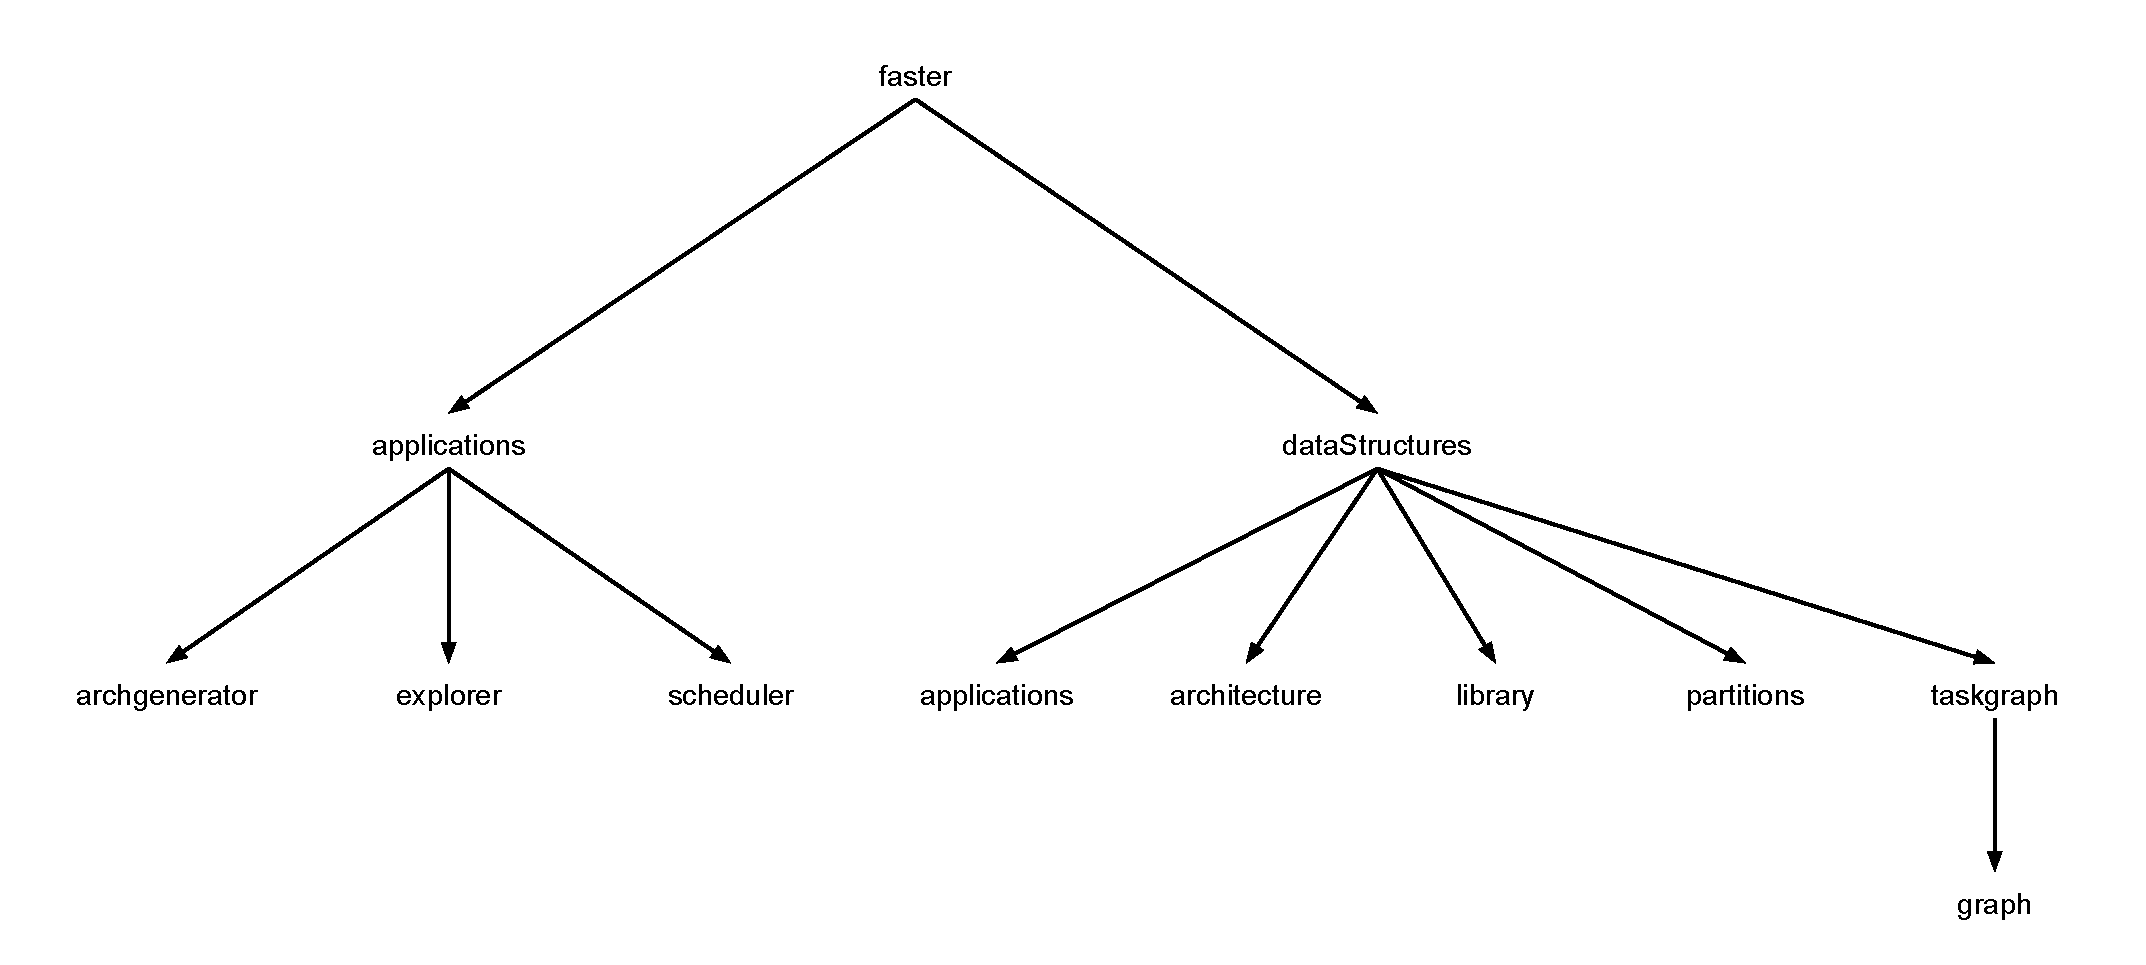
\includegraphics[width=\textwidth]{capitoli/figure/cap5/FASTERNamespaces.pdf}
\caption{Gerarchia dei namespace di \acs{FASTER}.}
\label{fig:gerarchiaNamespace}
 \end{center}
\end{figure}

Una rappresentazione della struttura dei namespace è visibile in figura 
\ref{fig:gerarchiaNamespace}. La maggior parte di questi namespace verrà 
spiegata al momento in cui saranno descritte classi o strutture che ne fanno parte 
e sono rilevanti per il lavoro oggetto della tesi.

\paragraph{Convenzioni nell'assegnazione dei nomi}
È stata scelta la seguente convenzione per nominare i dati membro o i metodi 
delle strutture/classi:
\begin{itemize}
 \item nomi di dati membro o metodi aventi specificatore di accesso 
\verb+public+ o \verb+protected+ sono scritti normalmente;
 \item nomi di dati membro o metodi aventi specificatore di accesso 
\verb+private+ sono scritti aggiungendo la stringa ``\verb+m_+'' come prefisso.
\end{itemize}

Eventuali tipi di dato ridefiniti tramite l'uso di \verb+typedef+ iniziano 
con una lettera maiuscola e sono scritti aggiungendo la stringa ``\verb+_t+'' 
come suffisso.

\paragraph{Puntatori e librerie esterne}
Allo scopo di prevenire il verificarsi di \emph{memory leak} difficili da 
identificare e debuggare, si è deciso all'inizio della progettazione di non 
utilizzare i puntatori standard forniti dal linguaggio C++, in favore degli 
shared pointer delle librerie \emph{Boost} \cite{BoostLibrary, BoostSharedPtr}.
Infatti, un oggetto di tipo \verb+boost::shared_ptr+ gestisce automaticamente 
la distruzione dell'oggetto a cui si riferisce una volta che l'ultimo shared 
pointer che punta all'oggetto è distrutto.

L'utilizzo degli shared pointer permette di istanziare l'oggetto tramite 
allocazione dinamica una sola volta, utilizzando poi i puntatori associati per 
l'accesso ai suoi dati e metodi, o per il passaggio come parametro.

Nel codice sorgente della toolchain sono presenti delle \verb+typedef+ globali 
aventi il suffisso ``\verb+Ptr+'' che semplificano la definizione degli shared 
pointer per alcune strutture/classi del progetto; ad esempio, alla classe 
\verb+FasterTask+, che identifica un task (generico) corrisponde lo shared 
pointer \verb+FasterTaskPtr+.

% TODO parlare di compilazione, CMake e librerie

\section{Strutture dati}
\label{sec:struttureDati}
In questa sezione vengono presentate alcune strutture dati della toolchain. La 
sezione si divide in due sotto-sezioni: la sezione 
\ref{subsec:struttureDatiMapper} presenta le strutture dati dell'algoritmo
evolvibile di esplorazione dello spazio delle soluzioni, non relative allo scheduler; la sezione 
\ref{subsec:struttureDatiScheduler} presenta invece le strutture utilizzate 
dall'algoritmo di scheduling.


\subsection{Algoritmo di esplorazione}
\label{subsec:struttureDatiMapper}
Questa sezione presenta le strutture dati di input e di output dell'algoritmo
di esplorazione, che si trovano nella cartella
\emph{toolchain/sources/common/datastructures/cpp/fasterInterfaces/explorer}
e appartengono al namespace \verb+faster::applications::explorer+.

\subsubsection{Input}
La \verb+struct+ che contiene i dati di input dell'algoritmo di esplorazione
\`e dichiarata e definita nei file \emph{explorerInput.hpp} e \emph{explorerInput.cpp},
rispettivamente.

La struttura \verb+ExplorerInput+ contiene il puntatore a una classe che incapsula i dati relativi al
progetto correntemente aperto in \ac{FASTER}, l'insieme dei parametri dell'algoritmo di
iterazione e l'insieme delle metriche e delle funzioni per valutarle.

\subsubsection{Lista dei mapping}
La struct \verb+ExplorerTrace+, dichiarata e definita nei file \emph{explorerTrace.hpp}
e \emph{explorerTrace.cpp}, contiene la lista delle triple
$<$\emph{task, processing element, implementazione}$>$ che viene calcolata da ogni
formica durante l'esplorazione, con i metodi per aggiungere un record
alla lista.

\subsubsection{Output}
La struct \verb+ExplorerOutput+, dichiarata e definita nei file \emph{explorerOutput.hpp}
e \emph{explorerOutput.cpp} contiene i valori associati a ciascuna metrica, il valore della funzione
obiettivo per la soluzione corrente, l'output dello scheduler (descritto in seguito) relativo
al mapping e le informazioni sull'evoluzione dell'area e del numero di processing element
utilizzati.

\subsection{Scheduler}
\label{subsec:struttureDatiScheduler}
L'obiettivo di questa sezione è presentare le più importanti strutture dati 
utilizzate dallo scheduler, che si trovano nella cartella 
\emph{toolchain/sources/common/datastructures/cpp/fasterInterfaces/scheduler}. 
Tutte le strutture che saranno esaminate in questa sezione appartengono al 
namespace \verb+faster::applications::scheduler+.

\subsubsection{Scheduler input}
I file \emph{schedulerInput.hpp} e \emph{schedulerInput.cpp} contengono la 
dichiarazione e l'implementazione della struttura \verb+SchedulerInput+, 
rispettivamente.

% Il seguente frammento di codice mostra le parti rilevanti della 
% dichiarazione della struttura.
% \newline
% \begin{minted}[baselinestretch=1,frame=single,fontsize=\footnotesize,gobble=2,
% mathescape]{c}
%   struct SchedulerInput {
%   private:
%       FasterProjectPtr m_fasterProject;
%       explorer::ExplorerTrace m_explorerTrace;
%       std::vector<FasterTaskPtr> m_topologicalSorting;
%       CriticalPathInfoMap_t m_criticalPathInfo;
%       std::vector<ProcessingTaskPair_t> m_reconfigurationsList;
%       bool m_busAvailable;
%       FasterTaskGraphPtr m_taskGraph;
%       FasterReconfigurationElementPtr m_reconfigurationController;
%       FasterMemoryElementPtr m_ramElement;
%       FasterCommunicationElementPtr m_busElement;
%       SchedulerMemoryManagerPtr m_memoryManager;
%       int m_readPortsNum;
%       int m_writePortsNum;
%       // code...
%   };
% \end{minted}
La struttura \verb+SchedulerInput+ contiene i dati principali che vengono usati 
dallo scheduler nel corso dell'elaborazione, dal preprocessing allo scheduling 
effettivo. In particolare, la struttura contiene il task graph dell'applicazione,
che viene arricchito durante la fase di scheduling, e la lista di triple calcolata
dal mapper per l'iterazione corrente dell'esplorazione.

Oltre a questi, vi sono anche dei puntatori al gestore della memoria e ai 
componenti di riconfigurazione e di comunicazione (\acs{RAM} e BUS, se 
presente), il numero di porte di lettura/scrittura disponibili sulla \acs{RAM} 
e variabili aggiuntive che contengono le informazioni di percorso critico dei 
task, l'ordinamento topologico dei task e la lista delle riconfigurazioni.

\subsubsection{Scheduler Data}
I file \emph{schedulerData.hpp} e \emph{schedulerData.cpp} contengono il codice 
sorgente della struttura \verb+SchedulerData+, che memorizza dati continuamente 
aggiornati durante l'esecuzione dell'algoritmo di scheduling. A differenza dei 
dati contenuti in \verb+SchedulerInput+, questi dati sono racchiusi in una 
struttura a sé stante perchè figurino come logicamente separati dai dati che 
invece fanno parte dell'input dell'algoritmo. La dichiarazione della struttura è
inclusa nel namespace \verb+faster::applications::scheduler::data+.

La struttura contiene l'insieme dei task non ancora 
selezionati per lo scheduling e i vettori dei task già schedulati e pronti per 
essere schedulati. Si è deciso di incapsulare questi dati in una struttura 
modificabile da tutti i componenti dell'algoritmo perchè alcuni componenti 
potrebbero dover fare delle modifiche on-the-fly.\footnote{Ad esempio, nel caso 
la policy di scheduling delle comunicazioni scelga di utilizzare il BUS come 
mezzo di comunicazione, il task \emph{READ} corrispondente dev'essere 
eliminato dalla lista dei task rimanenti.}

\subsubsection{Scheduler Gantt}
La struttura \verb+SchedulerGantt+ è definita nei file 
\emph{schedulerGantt.hpp} e \emph{schedulerGantt.cpp}; la struttura contiene il 
diagramma di Gantt utilizzato dall'algoritmo per visualizzare la soluzione 
calcolata. All'inizio dell'elaborazione il diagramma è vuoto, viene 
progressivamente riempito con le informazioni di scheduling calcolate ad ogni 
passo.

Sono a disposizione dei metodi pubblici per aggiungere le informazioni di 
scheduling relative a un task, per verificare se un determinato componente è 
occupato in un determinato istante di tempo e per ottenere il primo istante di 
tempo in cui un determinato componente è libero.

\subsubsection{Scheduler Output}
I file \emph{schedulerOutput.hpp} e \emph{schedulerOutput.cpp} contengono la 
dichiarazione e la definizione della struttura \verb+SchedulerOutput+. Questa 
struttura contiene i dati di output dello scheduler, che vengono 
progressivamente aggiornati man mano che l'esecuzione dell'algoritmo avanza, e 
alla fine sono utilizzati per il calcolo della metrica \emph{makespan}.

La struttura agisce come wrapper attorno ai 
metodi della struttura \verb+SchedulerGantt+ vista in precedenza, ed espone dei 
metodi che permettono di aggiungere all'output le informazioni appena calcolate.
Il metodo \verb+computeMakespan()+ permette di calcolare la metrica di valutazione
dello scheduling.

\subsubsection{Scheduler Utility}
I file \emph{schedulerUtility.hpp} e \emph{schedulerUtility.cpp}, infine, 
contengono la definizione di alcune strutture comunemente utilizzate dallo 
scheduler.

La struttura \verb+TaskTimes+ incapsula gli istanti di inizio e fine di un task.
\newline
\begin{minted}[baselinestretch=1,frame=single,fontsize=\footnotesize,gobble=2,
mathescape]{c}
  struct TaskTimes {
      long int startTime;
      long int endTime;
      // constructor, destructor and operators
  };
\end{minted}

La struttura \verb+CriticalPathInfo+ contiene le informazioni relative al 
percorso critico di un task.
\newline
\begin{minted}[baselinestretch=1,frame=single,fontsize=\footnotesize,gobble=2,
mathescape]{c}
  struct CriticalPathInfo {
      long int asap;
      long int alap;
      long int slack;
  };
\end{minted}

La struttura \verb+ScheduledTaskInfo+ contiene le informazioni riguardanti lo 
scheduling di un task.
\newline
\begin{minted}[baselinestretch=1,frame=single,fontsize=\footnotesize,gobble=2,
mathescape]{c}
  struct ScheduledTaskInfo {
      FasterTaskPtr task;
      FasterImplementationPtr implementation;
      FasterComponentPtr component;
      TaskTimes times_info;
      long int executionTime;
      // operators
  };
\end{minted}

La struttura \verb+MemoryOccupationInfo+ contiene le informazioni relative a 
un'area di memoria che viene allocata a un processing task.
\newline
\begin{minted}[baselinestretch=1,frame=single,fontsize=\footnotesize,gobble=2,
mathescape]{c}
  struct MemoryOccupationInfo {
      unsigned long base_addr;
      unsigned long data_size;
      TaskSet_t consumersSet;
      bool reusable_area;
  };
\end{minted}

% Infine, all'interno del file \emph{schedulerUtility.cpp} è presente un 
% namespace \verb+utilities+, che contiene due strutture che hanno l'operatore 
% \verb+()+ ridefinito. Queste strutture vengono utilizzate per testare 
% l'equivalenza o per calcolare l'hash di un oggetto del tipo specificato tramite 
% template. Vengono utilizzate nelle mappe e negli insiemi non ordinati mostrati 
% nelle strutture precedenti, e operano sul dato membro ``\verb+id+'' 
% dell'oggetto passato come parametro.


\section{Classi e gerarchie principali}
\label{sec:classiGerarchie}
In questa sezione vengono presentate le classi principali della toolchain 
relativa all'algoritmo di esplorazione (mapper) e dell'algoritmo di scheduling
utilizzato per la valutazione quantitativa della soluzione proposta dal mapper.

\subsection{Algoritmo di esplorazione}
\label{subsec:algoritmoEsplorazione}
Il codice sorgente dell'algoritmo di esplorazione è localizzato nella cartella 
\emph{toolchain/sources/explorer}. L'eseguibile dell'algoritmo di esplorazione 
è compilato a partire dal \verb+main()+ che si trova nel file sorgente 
\emph{explorerMain.cpp} nella suddetta cartella. Il main si occupa di 
istanziare i vari componenti che verranno spiegati nelle prossime sezioni e di 
lanciare la procedura di esplorazione. Al termine, viene generato un file di 
output e stampate le statistiche dell'esplorazione.

\subsubsection{Componente di esplorazione}
Il componente di esplorazione viene istanziato dalla funzione \verb+main()+ e 
si occupa di gestire l'esplorazione dal momento del lancio, effettuato nel main, 
fino alla terminazione. Il codice di questo componente è contenuto nei file 
\emph{explore.hpp} ed \emph{explore.cpp}, presenti nella sottocartella 
\emph{explore}.


Poichè il componente di esplorazione rappresenta un oggetto contenente un 
algoritmo invocabile, secondo la convenzione definita nella sezione
\ref{sec:osservazioniGenerali}, è implementato come \verb+class+ e 
inserito nel namespace \verb+faster::applications::explorer+, come tutti i 
componenti che vedremo di seguito relativi all'algoritmo di esplorazione.


\subsubsection{Componente di iterazione}
Data l'ampia modularità decisa in fase di progettazione, il componente di 
iterazione è rappresentato da una classe astratta che espone 
\verb+nextIteration()+, un metodo virtuale puro\footnote{Un metodo virtuale 
puro deve essere implementato da tutte le sottoclassi della classe che lo 
dichiara.} che si occupa di gestire un'iterazione dell'esplorazione.

L'interfaccia della classe astratta è definita in 
\emph{explore/exploreComponents/iteration/exploreIterationAlgorithm.hpp}; è 
presente anche una sottoclasse che implementa la funzionalità iterativa, nella 
sottocartella \emph{explore/exploreComponents/iteration/aco}. In ogni caso si 
può estendere aggiungendo altri componenti come sottoclassi separate che 
ridefiniscono il metodo per l'iterazione.
\newline
\begin{minted}[baselinestretch=1,frame=single,fontsize=\footnotesize,gobble=2,
mathescape]{c}
  class ExploreIterationAlgorithm {
      protected:
          const ExplorerInput& m_explorerInput;
      public:
          // constructor and destructor
          virtual std::set<ExplorerOutput> nextIteration() = 0;
          virtual ExplorerOutput getCurrentBestSolution() const = 0;
          virtual std::set<ExplorerOutput> getLastIterationSolutions()
              const = 0;
  };
\end{minted}

La sottoclasse \verb+ExploreIterationACO+, dichiarata e definita nei file
\emph{exploreIterationACO.hpp} e \emph{exploreIterationACO.cpp} implementa
l'iterazione della metodologia descritta nel capitolo \ref{chap:approccio}.
\newline
\begin{minted}[baselinestretch=1,frame=single,fontsize=\footnotesize,gobble=2,
mathescape]{c}
  for (unsigned long int antNumber=0; antNumber<m_antsPerGeneration; antNumber++)
  {
      // code...
      std::map<FasterProcessingTaskPtr, double> tasksProbabilityMap;
      std::map<FasterProcessingTaskPtr, double> localHeuristicPerTaskMap;
      for (const FasterProcessingTaskPtr &taskIter : readyTasksSet)
      {
          tasksProbabilityMap = m_computeProbabilityNextTask(m_alphaTask,
              m_betaTask, localHeuristicPerTaskMap);
          FasterProcessingTaskPtr theOneTask =
              m_rouletteWheelSelection(tasksProbabilityMap);
          // code...
          for (const FasterImplementationPtr &i :
               m_fasterProject->getImplementationPtrsSetGivenProcessingTask
               (theOneTask))
          {
              // compute local heuristics for processing elements
          }
          std::pair<FasterProcessorPtr, FasterImplementationPtr>
              theOneProcessorAndImplementation =
              m_rouletteWheelSelection(processorAndImplementationProbabilityMap);
      }
      // construct mapping and invoke scheduler to obtain makespan
      // metric value
  }
  m_thisGenerationBestSolutionsSet =
      m_selectBestSolutions(m_thisGenerationSolutionsSet);
  m_updateGlobalPheromoneMatrix(m_thisGenerationSolutionsSet,
      m_thisGenerationBestSolutionsSet);
  // return this generation's best solutions
  return m_thisGenerationBestSolutionsSet;
\end{minted}


\subsubsection{Componente di terminazione}
La terminazione dell'algoritmo di esplorazione viene decisa dal componente di 
terminazione. Come per l'iterazione, anche il componente di iterazione è 
composto da una classe astratta che espone un metodo che deve essere 
reimplementato dalle sottoclassi, \verb+isTerminated()+.

Come nel caso del componente di iterazione, è presente un'implementazione della 
classe astratta, che termina quando il numero di iterazioni raggiunge il limite 
specificato nel file di configurazione dell'algoritmo.
\newline
\begin{minted}[baselinestretch=1,frame=single,fontsize=\footnotesize,gobble=2,
mathescape]{c}
  class ExploreTerminationAlgorithm {
      protected:
          const ExplorerInput & m_sd;
      public:
          // constructor and destructor
          virtual bool isTerminated() const = 0;
          virtual void updateState(std::set<ExplorerOutput>) = 0;
          virtual faster::dataStructures::FasterPerformanceStatistics 
              getStatistics() = 0;
  };
\end{minted}

% TODO metriche dell'algoritmo di esplorazione

\subsection{Algoritmo di scheduling}
\label{subsec:algoritmoScheduling}
L'obiettivo di questa sezione è presentare le porzioni più importanti del 
codice dell'algoritmo di scheduling. Le interfacce di input/output e le 
strutture dati utilizzate sono già state descritte nella sezione 
\ref{subsec:struttureDatiScheduler}, mentre in questa sezione verranno esaminati i 
vari componenti dello scheduler che gestiscono l'elaborazione.

Il codice sorgente dell'algoritmo di scheduling è contenuto nella cartella 
\emph{toolchain/sources/scheduler}; la sua struttura rispecchia quella 
dell'algoritmo di esplorazione, come verrà spiegato nelle prossime sezioni per 
l'esame dei componenti dello scheduler. Tutte le classi che compongono 
sono incluse nel namespace \verb+faster::applications::scheduler+.

\subsubsection{Componente di scheduling}
La sottocartella \emph{schedule} contiene la dichiarazione e definizione di
\verb+Schedule+, una classe astratta che espone un metodo virtuale puro per il 
calcolo dello scheduling. In questo modo è possibile utilizzare algoritmi 
completamente differenti semplicemente creando una nuova sottoclasse di 
\verb+Schedule+ che implementa il metodo \verb+computeSchedule()+.
\newline
% FIXME perchè c'è m_explorerInput dentro???
\begin{minted}[baselinestretch=1,frame=single,fontsize=\footnotesize,gobble=2,
mathescape]{c}
  class Schedule {
      protected:
          const explorer::ExplorerInput & m_explorerInput;
          SchedulerOutput m_schedulerOutput;
      public:
          // code
          virtual SchedulerOutput computeSchedule(
                  const explorer::ExplorerTrace & trace) = 0;
  };
\end{minted}

La sottoclasse che implementa lo scheduler seguendo l'approccio descritto nel capitolo 
\ref{chap:approccio}, è chiamata \verb+ScheduleRB+ ed è contenuta nella 
sottocartella \emph{schedule/scheduleComponents}. Nel seguente frammento 
vengono riportate le parti rilevanti della dichiarazione della classe, con 
l'inclusione dei vari componenti.
\newline
\begin{minted}[baselinestretch=1,frame=single,fontsize=\footnotesize,gobble=2,
mathescape]{c}
  class ScheduleRB : public Schedule {
    private:
      SchedulerInput m_schedulerInput;
      SchedulerBestSchedulableTaskAlgorithmPtr m_bestSchedulableAlgorithm;
      SchedulerTimeAssignmentAlgorithmPtr m_timeAssignmentAlgorithm;
      data::SchedulerData m_schedulerData;
      // code...
    public:
      // code...
      virtual SchedulerOutput computeSchedule(
              const explorer::ExplorerTrace & trace);
  };
\end{minted}

Viene di seguito presentato il core loop dell'algoritmo di scheduling.
\newline
\begin{minted}[baselinestretch=1,frame=single,fontsize=\footnotesize,gobble=2,
mathescape]{c}
  // code...
  ScheduleRBAnalyzeTrace preprocessingAlgorithm(m_schedulerInput);
  preprocessingAlgorithm.doPreprocessing();
  // code...
  do {
    m_resolveDependencies();
    FasterTaskPtr bestTask;
    bestTask = m_bestSchedulableAlgorithm->bestSchedulableTask(
               m_schedulerData.readyTasksList);
    // code...
    ScheduledTaskInfo taskInfo;
    taskInfo = m_timeAssignmentAlgorithm->calculateSchedulingInfo(bestTask);
    m_schedulerData.scheduledTasksList.push_back(bestTask);
    m_lastScheduledTask = bestTask;
    m_schedulerOutput.addScheduledTaskInfo(bestTask, taskInfo);
    m_schedulerData.readyTasksList.erase(
                        std::find(m_schedulerData.readyTasksList.begin(), 
                        m_schedulerData.readyTasksList.end(), bestTask));
    m_schedulerData.unscheduledTasksSet.erase(bestTask);
  } while (!m_schedulerData.unscheduledTasksSet.empty());
\end{minted}

Il metodo \verb+m_resolveDependencies()+ riempie la lista di task pronti per 
essere schedulati con i task che hanno tutte le precedenze soddisfatte; come si 
può vedere dal frammento di codice precedente, il task migliore tra quelli 
pronti viene selezionato da un componente dedicato alla selezione dei task e 
schedulato da un altro componente dedicato all'assegnazione dei tempi. Una 
volta che le informazioni di scheduling per il task selezionato sono state 
calcolate, il task è considerato come schedulato, le informazioni sono aggiunte 
all'output (metodo \verb+addScheduledTaskInfo()+) e il task è rimosso dalla 
lista ``ready'' e dall'insieme dei task non ancora schedulati. Il ciclo è 
ripetuto fino a che vi sono task non schedulati.

\subsubsection{Componente di preprocessing}
Il codice del componente dedicato al preprocessing è contenuto nella 
sottocartella \emph{schedule/scheduleComponents/preprocessing}; la classe 
\verb+ScheduleRBPreprocessingAlgorithm+ è una classe astratta che espone un 
metodo virtuale puro da reimplementare per poter personalizzare la fase di 
preprocessing. La sottoclasse \verb+ScheduleRBAnalyzeTrace+ ne fornisce 
un'implementazione, che è quella utilizzata nell'algoritmo di scheduling 
trattato in questa tesi e descritta ad alto livello nella sezione 
\ref{subsec:fasePreprocessing}.
\newline
\begin{minted}[baselinestretch=1,frame=single,fontsize=\footnotesize,gobble=2,
mathescape ]{c}
  void ScheduleRBAnalyzeTrace::doPreprocessing()
  {
    std::vector<explorer::ExplorerTraceStep_t> traceSteps = 
        m_schedulerInput.getExplorerTrace().getTrace();
    m_taskGraph = 
      m_schedulerInput.getFasterProject()->getPartition(0)->taskgraph->clone();
    m_integrateCommunications(traceSteps);
    m_integrateReconfigurations(traceSteps);
    m_schedulerInput.setTaskGraph(m_taskGraph);
    m_schedulerInput.setReconfigurations(m_reconfigurationsList);
    m_computeCriticalPathInfo();
  }
\end{minted}

Come si può vedere dal codice, la fase di preprocessing clona il task graph 
originale del progetto, lo modifica di conseguenza integrando comunicazioni e 
riconfigurazioni e lo imposta come input dell'algoritmo di scheduling.

\subsubsection{Componente di scelta dei task}
Il codice del componente di scelta dei task è contenuto nella sottocartella 
\emph{schedule/scheduleComponents/bestTaskAlgorithm}; il suo compito è 
implementare un generico metodo di scelta dei task. In maniera simile ai 
componenti precedentemente descritti, esiste una classe astratta base 
\verb+SchedulerBestSchedulableTaskAlgorithm+ che contiene il metodo virtuale 
puro \verb+bestSchedulableTask()+, che dev'essere reimplementato dalle 
sottoclassi nel caso si voglia utilizzare un diverso criterio di scelta dei 
task.
\newline
\begin{minted}[baselinestretch=1,frame=single,fontsize=\footnotesize,gobble=2,
mathescape]{c}
  class SchedulerBestSchedulableTaskAlgorithm {
    protected:
      const SchedulerInput & m_schedulerInput;
    public:
      // constructor and destructor
      virtual FasterTaskPtr bestSchedulableTask(
              const std::vector<FasterTaskPtr> & readyList) const = 0;
  };
\end{minted}

La sottoclasse di \verb+SchedulerBestSchedulableTaskAlgorithm+
che implementa il metodo come visto nella sezione \ref{sec:euristicaSceltaTask}
è chiamata \verb+ScheduleRBPriorityHeuristic+ e si trova nella sottocartella 
\emph{schedule/scheduleComponents/bestTaskAlgorithm/priorityHeuristic} ed è 
dichiarata e definita nei file \emph{scheduleRBPriorityHeuristic.hpp} e 
\emph{scheduleRBPriorityHeuristic.cpp}.
\newline
\begin{minted}[baselinestretch=1,frame=single,fontsize=\footnotesize,gobble=2,
mathescape]{c}
  struct PriorityMetrics {
    FasterTaskPtr task;
    float longestPath;
    float est;
    float eft;
  };
  class ScheduleRBPriorityHeuristic : public 
          SchedulerBestSchedulableTaskAlgorithm {
    private:
      enum PriorityFunctionParameters {
              LP = 10,
              EST = 5,
              EFT = 2,
              WriteBeforeReconfiguration = 50
      };
      // code...
      mutable float m_decayFactor;
    public:
      // constructor and destructor
      virtual FasterTaskPtr bestSchedulableTask(
              const std::vector<FasterTaskPtr> & readyList) const;
  };
\end{minted}

Nel frammento di codice è inclusa la dichiarazione della 
struttura \verb+PriorityMetrics+, che contiene le tre metriche utilizzate per 
il calcolo della priorità di un task.

All'interno della classe che implementa l'euristica si trovano invece i 
parametri (pesi) assegnati alle varie metriche e il boost di priorità assegnato 
ai task di comunicazione di tipo \emph{WRITE} che precedono una 
riconfigurazione, nella enum \verb+PriorityFunctionParameters+. Il dato membro 
\verb+m_decayFactor+ rappresenta il fattore di degrado che riduce la cifra di 
merito corrispondente alle informazioni sul percorso critico.

Viene ora presentato il codice della funzione che inizializza i valori delle 
metriche nella struttura, con le relative funzioni per il calcolo delle singole 
metriche.
\newline
\begin{minted}[baselinestretch=1,frame=single,fontsize=\footnotesize,gobble=2,
mathescape]{c}
  PriorityMetrics ScheduleRBPriorityHeuristic::m_computePriorityMetrics(const 
                      FasterTaskPtr & task, bool isSoftCoreMapped) const
  {
    PriorityMetrics metrics;
    metrics.task = task;
    if (isSoftCoreMapped) {
      metrics.longestPath = m_computeLongestPath(task);
    } else {
      metrics.longestPath = m_computeLongestPath(task);
      metrics.est = m_computeEST(task);
      metrics.eft = m_computeEFT(task);
    }
    return metrics;
  }
  // ...
  float ScheduleRBPriorityHeuristic::m_computeLongestPath(
        const FasterTaskPtr & task) const
  {
    const CriticalPathInfoMap_t & criticalPathInfo = 
            m_schedulerInput.getCriticalPathInfo();
    CriticalPathInfo info = criticalPathInfo.find(task)->second;
    long int slack = info.slack;
    if (slack >= 0 && slack <= SLACK_THRESHOLD) {
      return PRIORITY_MAX * m_decayFactor;
    }
    float logSlack = ::log2(slack);
    return 1 / logSlack;
  }
  // ...
  float ScheduleRBPriorityHeuristic::m_computeEST(
        const FasterTaskPtr & task) const
  {
    const CriticalPathInfoMap_t & criticalPathInfo = 
            m_schedulerInput.getCriticalPathInfo();
    CriticalPathInfo info = criticalPathInfo.find(task)->second;
    return info.asap == 0 ? info.asap : ::log2(info.asap);
  }
  // ...
  float ScheduleRBPriorityHeuristic::m_computeEFT(
        const FasterTaskPtr & task) const
  {
    const CriticalPathInfoMap_t & criticalPathInfo = 
          m_schedulerInput.getCriticalPathInfo();
    CriticalPathInfo info = criticalPathInfo.find(task)->second;
    long int asap = info.asap;
    long int execTime = m_helperAlgorithms.computeExecTime(task);
    return ::log2(asap + execTime);
  }
\end{minted}


\subsubsection{Componente di assegnazione dei tempi}
Il componente dell'algoritmo di scheduling che gestisce l'assegnazione dei 
tempi è contenuto nella sottocartella 
\emph{schedule/scheduleComponents/timeAssignmentAlgorithm}; il suo compito è 
implementare la policy di assegnazione dei tempi ai vari task che vengono via 
via selezionati. La classe astratta \verb+SchedulerTimeAssignmentAlgorithm+ 
contiene un metodo virtuale puro che viene reimplementato dalle sottoclassi.
\newline
\begin{minted}[baselinestretch=1,frame=single,fontsize=\footnotesize,gobble=2,
mathescape]{c}
  class SchedulerTimeAssignmentAlgorithm {
    protected:
      const SchedulerInput & m_schedulerInput;
    public:
      // constructor and destructor
      virtual ScheduledTaskInfo calculateSchedulingInfo(
              const FasterTaskPtr & task) const = 0;
  };
\end{minted}

La sottoclasse che implementa il metodo nell'algoritmo trattato in questa tesi 
è chiamata \verb+ScheduleRBASAPAlgorithm+, nel seguente frammento di codice ne 
è illustrata la dichiarazione.
\newline
\begin{minted}[baselinestretch=1,frame=single,fontsize=\footnotesize,gobble=2,
mathescape]{c}
  class ScheduleRBASAPAlgorithm : public SchedulerTimeAssignmentAlgorithm {
    private:
      // code...
      ScheduledTaskInfo m_calculateSchedulingInfoProcessingTask(
                        const FasterTaskPtr & procTask) const;
      ScheduledTaskInfo m_calculateSchedulingInfoCommunicationTask(
                        const FasterTaskPtr & commTask) const;
      ScheduledTaskInfo m_calculateSchedulingInfoReconfigurationTask(
                        const FasterTaskPtr & reconfTask) const;
      ScheduledTaskInfo m_calculateSchedulingInfoCommWriteTask(
                        const FasterCommunicationWriteTaskPtr & commWriteTask) const;
      ScheduledTaskInfo m_calculateSchedulingInfoCommReadTask(
                        const FasterCommunicationReadTaskPtr & commReadTask) const;
      void m_allocateMemoryForTask(const FasterTaskPtr & task) const;
      // code...
    public:
      // constructor and destructor
      virtual ScheduledTaskInfo calculateSchedulingInfo(
              const FasterTaskPtr & task);
  };
\end{minted}
Dal codice precedente è possibile vedere le dichiarazioni dei metodi che 
calcolano le informazioni di scheduling per le tre principali categorie di 
task e per i due tipi di task di comunicazione. Al momento di effettuare lo 
scheduling di un task di comunicazione, viene istanziato l'oggetto che 
implementa la policy di scheduling delle comunicazioni.

Il metodo \verb+m_allocateMemoryForTask()+ gestisce l'allocazione della memoria 
per i task di computazione chiamando i metodi del gestore della memoria.

\paragraph{Policy di scheduling delle comunicazioni}
La classe \verb+ScheduleRBCommunicationPolicy+ gestisce lo scheduling dei task 
di comunicazione e implementa la policy spiegata nella sezione 
\ref{subsec:policyComunicazioni}. La classe è dichiarata e definita nei file 
\emph{scheduleRBCommunicationPolicy.hpp} e  \emph{scheduleRBCommunicationPolicy.cpp},
contenuti nella sottocartella  \emph{schedule/scheduleComponents/timeAssignmentAlgorithm/asap/communicationPolicy}.
\newline
\begin{minted}[baselinestretch=1,frame=single,fontsize=\footnotesize,gobble=2,
mathescape]{c}
  class ScheduleRBCommunicationPolicy {
    public:
      // code...
      ScheduledTaskInfo scheduleCommunicationTask(
                        const FasterCommunicationTaskPtr & commTask, long int precTime);
    private:
      void m_removeConsumers(
           const FasterCommunicationTaskPtr & commTask, bool scheduledOnBus);
      // other private members
  };
\end{minted}

Il metodo \verb+scheduleCommunicationTask()+ implementa la policy di scheduling dei
task di comunicazione vista nel capitolo precedente; una volta calcolate le informazioni
di scheduling, viene invocato il metodo \verb+m_removeConsumers()+ che si occupa di
eliminare il task target della comunicazione dalla lista dei task in attesa per
i dati presenti in memoria.

\subsubsection{Allocazione della memoria}
La classe \verb+SchedulerMemoryManager+, dichiarata e definita nei file
\emph{schedulerMemoryManager.hpp} e \emph{schedulerMemoryManager.cpp} contenuti nella cartella
\emph{toolchain/sources/common/datastructures/cpp/fasterInterfaces/scheduler}, gestisce
gestisce l'allocazione della memoria per i processing task che compongono l'applicazione.
\newline
\begin{minted}[baselinestretch=1,frame=single,fontsize=\footnotesize,gobble=2,mathescape]{c}
  typedef std::unordered_map<FasterTaskPtr, MemoryOccupationInfo,
          utilities::HashUtility<FasterTaskPtr> > MemoryOccupationMap_t;
  class SchedulerMemoryManager {
    public:
      // constructor and destructor
      void addMemoryInfo(
           const FasterTaskPtr & task,
           const MemoryOccupationInfo & info);
      void addMemoryInfo(
           const FasterTaskPtr & task,
           unsigned long base_addr,
           unsigned long data_size,
           TaskSet_t consumersSet);
      void allocateMemoryForTask(
           const FasterTaskPtr & task,
           unsigned long data_size,
           const TaskSet_t & consumersSet);
      void removeConsumer(const FasterTaskPtr & consumer);
      MemoryOccupationInfo getMemoryOccupationInfo(
                           const FasterTaskPtr & task) const;
      MemoryOccupationMap_t getMemoryOccupationMap() const;
      void setMemoryOccupationMap(const MemoryOccupationMap_t & map);
    private:
      unsigned long m_getFirstAvailableAddress(unsigned long data_size);          
      MemoryOccupationMap_t m_memoryOccupationMap;          
      unsigned long m_largestAvailableAddress;
  };
\end{minted}

La mappa \verb+m_memoryOccupationMap+ contiene le aree di memoria allocate per tutti i
task e i metodi necessari per riservare uno spazio di indirizzi a un nuovo task, oltre
al metodo per rimuovere un task di comunicazione (consumatore) dalla lista di task in
attesa dei dati contenuti nella memoria.
